\documentclass[11pt,a4paper]{article}
\usepackage[utf8]{inputenc}
\usepackage[spanish]{babel}
\usepackage{amsmath}
\usepackage{amsfonts}
\usepackage{amssymb}
\usepackage[export]{adjustbox}
\usepackage{tabularx}
\usepackage[table]{xcolor}
\usepackage{float}
\usepackage{url}
\usepackage{hyperref}
\hypersetup{
    colorlinks=true,
    linkcolor=black,
    filecolor=black,      
    urlcolor=blue,
    citecolor=blue,
}
\usepackage{graphicx}
\graphicspath{ {images/} }


\begin{document}


\begin{titlepage}

\includegraphics[scale=0.2,right,valign=t]{uoc-logo.png}
\vspace*{\fill}
\begin{flushleft}
{\LARGE \textbf{YouTubeCrawlerTool: Aplicación web para habilitar el estudio del movimiento antivacuna en YouTube}}
\end{flushleft}
\begin{flushleft}
\textbf{Javier Sánchez Mendoza}\\
Grado de ingeniería informática\\
Health IT
\end{flushleft}
\begin{flushleft}
\textbf{Carlos Luis Sánchez Bocanegra}\\
\textbf{José Antonio Morán Moreno}
\end{flushleft}
\begin{flushleft}
Junio de 2018  
\end{flushleft}
\end{titlepage}


\begin{titlepage}
\vspace*{\fill}
\begin{flushleft}

\includegraphics[scale=1,left]{licencia-cc.png}
Esta obra está sujeta a una licencia de\\
Reconocimiento-NoComercial-SinObraDerivada\\
\href{http://creativecommons.org/licenses/by-nc-nd/3.0/es/}{3.0 España de Creative Commons}
\end{flushleft}
\end{titlepage}



\begin{flushleft}
\textit{Quiero dedicar este trabajo especialmente a:}
\linebreak
 
\textbf{\textit{Carolina}} \\
\textit{Por empujarme a retomar mis estudios y, lo que es mas importante, motivarme durante todo este tiempo.}
\linebreak

\textbf{\textit{Amy, Luke y Jim}}\\
\textit{Por obligarme a salir a la calle de vez en cuando y estar siempre hay.}
\linebreak
\end{flushleft}
\newpage 



\begin{center}
\textbf{FICHA DEL TRABAJO FINAL}
\end{center}
\begin{tabularx}{\textwidth}{|X|X|}
\hline 
\textbf{Título del trabajo:} &\cellcolor{gray!25} \textit{YouTubeCrawlerTool: Aplicación web para habilitar el estudio del movimiento antivacuna en YouTube} \\ 
\hline 
\textbf{Nombre del autor:} &\cellcolor{gray!25} \textit{Javier Sánchez Mendoza} \\ 
\hline 
\textbf{Nombre del consultor/a:} &\cellcolor{gray!25} \textit{Carlos Luis Sánchez Bocanegra} \\ 
\hline 
\textbf{Nombre del PRA:} &\cellcolor{gray!25} \textit{José Antonio Morán Moreno} \\ 
\hline 
\textbf{Fecha de entrega:} &\cellcolor{gray!25} \textit{06/2018} \\ 
\hline 
\textbf{Titulación:} &\cellcolor{gray!25} \textit{Grado de ingeniería informática} \\ 
\hline 
\textbf{Área del Trabajo Final:} &\cellcolor{gray!25} \textit{Health IT} \\ 
\hline 
\textbf{Idioma del trabajo:} &\cellcolor{gray!25} \textit{Español} \\ 
\hline 
\textbf{Palabras clave:} &\cellcolor{gray!25} \textit{antivacuna, crawler, YouTube.} \\ 
\hline
\end{tabularx} 
\begin{tabularx}{\textwidth}{|X|}
\textbf{Resumen del Trabajo (máximo 250 palabras):} \textit{Con la finalidad, contexto de aplicación, metodología, resultados i conclusiones del trabajo.} \\ 
\hline 
\cellcolor{gray!25} \textit{...} \\
\hline 
\end{tabularx} 
\newpage 


\begin{tabularx}{\textwidth}{|X|}
\hline 
\textbf{Abstract (in English, 250 words or less):} \\ 
\hline 
\cellcolor{gray!25} \textit{...} \\
\hline 
\end{tabularx} 
\newpage 


\tableofcontents
\newpage


\listoffigures
\newpage


\section{Introducción}
En esta sección se detalla el proyecto, la motivación de la elección de la temática escogida y la planificación y estructuración del mismo.


\subsection{Contexto y justificación del Trabajo}
Desde la introducción de la vacunación como método preventivo de enfermedades han existido entidades y grupos de personas que se han opuesto a ella y han dudado de su efectividad o propósito \cite{1}. Hoy en día el activismo anti-vacunación (conocido también como movimiento antivacunas) ha vuelto a la actualidad y se encuentra en auge en algunas regiones tales como Europa o Estados Unidos, cobrándose en el peor de los escenarios victimas mortales a causa de enfermedades que se creían erradicadas y que han vuelto a surgir \cite{2}\cite{3}.
\linebreak

Para hacer posible el estudio y comprensión de las motivaciones del movimiento antivacuna y luchar contra su desinformación, se propone el desarrollo de una aplicación que permita la recolección de grandes cantidades de datos de la actividad realizada por parte de este colectivo en redes sociales con el fin de hacer posible su posterior tratamiento y estudio para obtener valor añadido. Para tal fin, en este proyecto contamos con la colaboración de Johanna Milena Rodríguez Vera estudiante de master en Telemedicina que asume el rol de analista de datos (\textit{data scientist} \cite{4}) en el desarrollo de su trabajo final de máster titulado \textit{Evaluación de la información sanitaria en vacunas disponible en las redes sociales - YouTube} y que actúa a la vez como clienta de la aplicación desarrollada en el presente proyecto.
\linebreak

Hoy en día las redes sociales han puesto al alcance de los analistas de datos una gran cantidad de información disponible para ser analizada, una de las problemáticas a las que se quiere hacer frente es la obtención de dichos datos de forma efectiva. Para ello se propone hacer uso de interfaces de programación de aplicaciones (abreviado como \textit{API} \cite{5} en ingles) ofrecidas públicamente por distintas redes sociales de tal forma que el proceso resulte transparente para el usuario final, permitiéndole la extracción a este problema.
\linebreak

La obtención de grandes volúmenes de datos nos lleva también a la problemática que surge en su almacenamiento en bases de datos tradicionales y su posterior procesamiento. Para habilitar al usuario final el correcto acceso a la información obtenida se estudían las ventajas que aporta el uso de bases de datos \textit{NoSQL} \cite{6} para este cometido, al ser diseñadas especialmente para manejar enormes cantidades de datos. Proyecto que se enmarca dentro de la problemática de la obtención, almacenamiento y procesamiento de grandes volúmenes de datos (\textit{Big Data} \cite{7}) y su posterior acceso.
\newpage

\subsection{Objetivos del Trabajo}
El objetivo principal del proyecto es proporcionar una aplicación web que permita a la clienta obtener de forma usable y transparente la información que necesite de la red social \textit{YouTube} para poder llevar a cabo el estudio de patrones de comportamiento entre las diferentes movimientos anti y pro vacuna.
\linebreak

Entre los objetivos secundarios del proyecto se encuentra la exploración de otras redes sociales y proporcionar una herramienta lo suficientemente genérica para que pueda ser utilizada en la investigación realizada por Johanna así como en otras investigaciones futuras de distinta temática.
\linebreak

Algunos objetivos concretos que se han querido lograr son los siguientes: 
\begin{itemize}
\item Investigar que funcionalidades aportan las \textit{API} públicas ofrecidas por \textit{YouTube} y analizar como se pueden utilizar para la obtención de la información requerida.
\item Determinar como almacenar y acceder de forma eficiente a la gran cantidad de información que se obtendrá.
\item Permitir la recolección de información según criterios de búsqueda proporcionados por el usuario final.
\item Habilitar la gestión, visualización y exportación de datos obtenidos en distintos procesos de extracción para su posterior análisis en herramientas especializadas.
\item Ofrecer herramientas de visualización para el análisis y comprensión de los datos obtenidos.
\item Proporcionar una interfaz de usuario usable que permita realizar las acciones requeridas por el usuario final.
\end{itemize}


\subsection{Enfoque y método seguido}
Para la realización del proyecto se ha seguido el marco ágil de desarrollo \textit{scrum} \cite{8}. Al adoptar esta metodología como marco de trabajo nos ha permitido, a diferencia de otras metodologías lineales de desarrollo como pueden ser los modelos en cascada, poder desarrollar el proyecto de forma flexible permitiéndonos adaptar la planificación inicial del proyecto en los casos necesarios para adecuarse a los nuevos requerimientos.
\\

La forma en la cual se aplico la metodología \textit{scrum} en el proyecto esta condicionada por los integrantes del equipo de desarrollo, en el cual la figura del \textit{product owner}, \textit{scrum master} y desarrollador recaen sobre la figura del alumno que presenta el actual proyecto descrito (Javier Sánchez Mendoza), mientras que la figura del cliente estará representada por una analista de datos (Johanna Milena Rodríguez Vera) y el consultor de los mismos (Carlos Luis Sánchez Bocanegra) como \textit{stakeholder}.
\\

Siguiendo la metodología \textit{scrum}, se realizaron iteraciones (comúnmente conocidos como \textit{sprints}) de una semana de duración donde, en la finalización de los mismos, se realizaron reuniones online para revisar y aprobar las tareas realizadas (\textit{sprint review}) y definir las tareas para la siguiente iteración (\textit{sprint planning}). Para gestionar las tareas a realizar (\textit{backlog}) se decidio utilizar la herramienta online \textit{Trello} \cite{9}:
\\

\begin{figure}[hbtp]
\centering
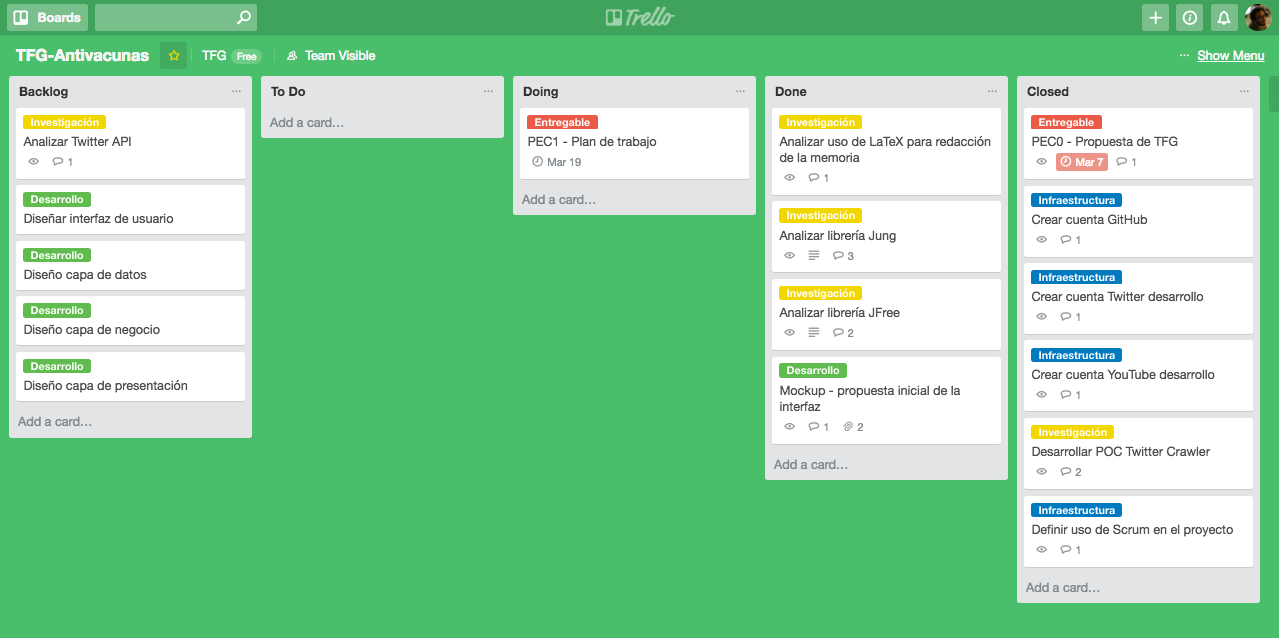
\includegraphics[scale=0.3]{planificacion/trello-backlog.png}
\caption{Ejemplo del backlog del proyecto en Trello}
\end{figure}


\subsection{Planificación del Trabajo}
En la realización del proyecto se propuso inicialmente seguir una planificación tentativa tal y como se detalla en el diagrama de \textit{Grantt} facilitado en las figuras dos y tres:

\begin{figure}[H]
\centering
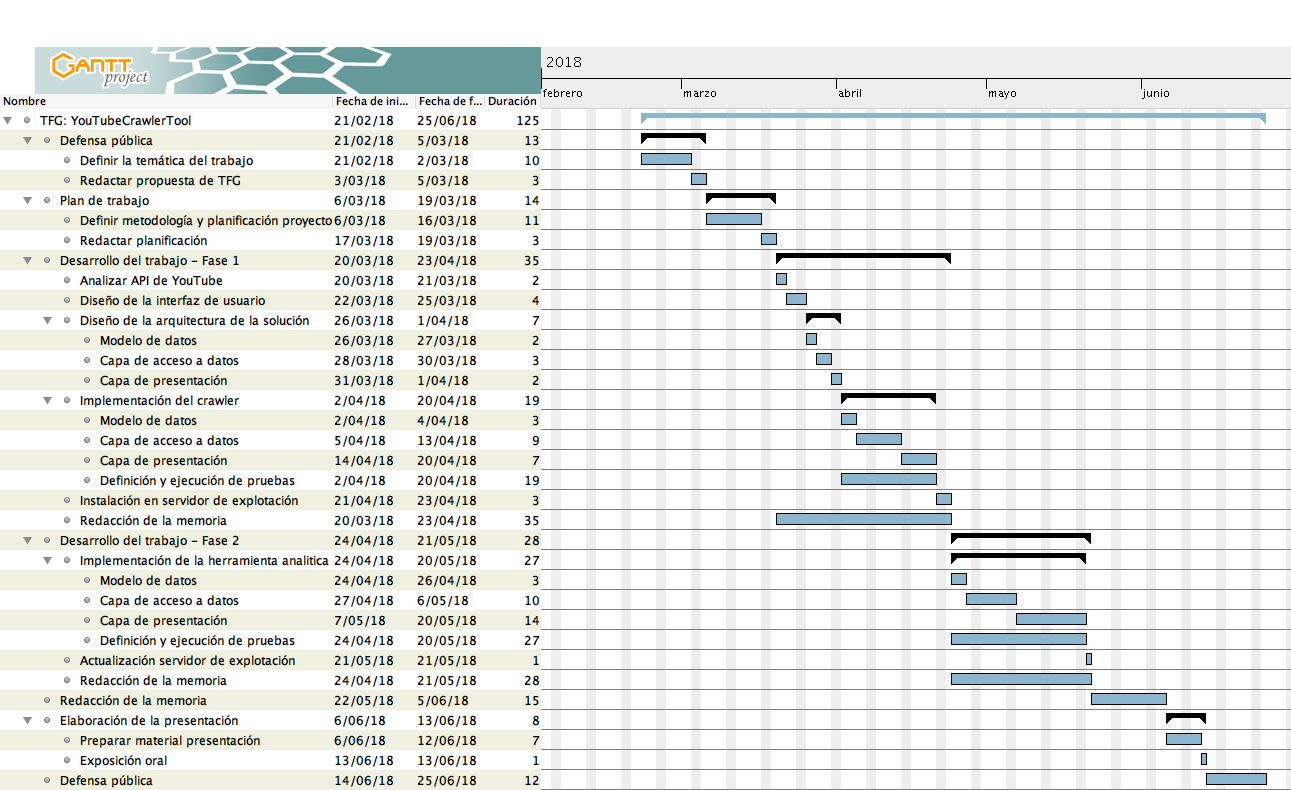
\includegraphics[scale=0.25]{planificacion/planificacion.png}
\caption{Listado de tareas y diagrama de Gantt}
\end{figure}

\begin{figure}[H]
\centering
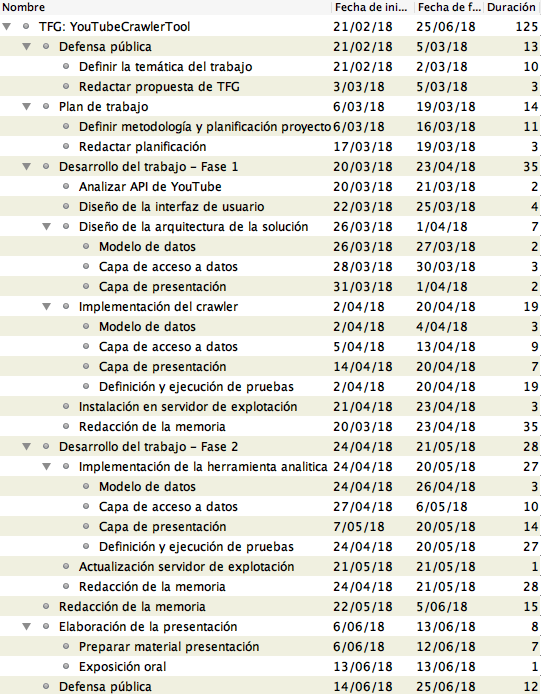
\includegraphics[scale=0.4]{planificacion/listado-tareas.png}
\caption{Listado de tareas}
\end{figure}
\newpage

De la planificación inicial cabe destacar que la redacción de la memoria se diseño como una tarea evolutiva que se desarrollaría durante todas las fases del proyecto pero mas intensamente durante la antepenúltima fase dedicada exclusivamente a su redacción. Además, durante las dos fases de desarrollo se  planificaron dos tareas recurrentes para la definición y realización de pruebas de calidad del producto a realizar durante todo el ciclo de desarrollo.
\linebreak

Como se puede observar, en el diagrama facilitado en cada entrega se pretendían conseguir unos hitos concretos. La relación de los mas destacables por entrega son los siguientes:

\begin{itemize}
\item \textbf{Definición de los contenidos del trabajo:} Redacción propuesta TFG.
\item \textbf{Plan de trabajo:} Redacción planificación.
\item \textbf{Desarrollo del trabajo – Fase 1:} Instalación en servidor de explotación de la primera versión de la aplicación con funcionalidad de \textit{crawler} implementada.
\item \textbf{Desarrollo del trabajo – Fase 2:} Actualización en servidor de explotación de la versión final de la aplicación con funcionalidad analítica implementada.
\item \textbf{Redacción de la memoria:} Entrega de la memoria del proyecto.
\item \textbf{Elaboración de la presentación:} Realizar exposición oral.
\item \textbf{Defensa pública:} Defender públicamente el proyecto.
\end{itemize}

Los riesgos detectados en la planificación inicial se concentraban principalmente en la consecución del hito definido en la primera fase de desarrollo. Para permitir a la clienta de la aplicación poder empezar a recopilar datos para su investigación lo antes posible, se decidió realizar la instalación de la aplicación desarrollada en un entorno de explotación en dos fases distintas, una con la funcionalidad del \textit{crawler} y otra con la funcionalidad analítica implementada. La demora en la primera fase de desarrollo podría comprometer el éxito de la investigación del cliente. Para mitigar este riesgo se realizo el seguimiento del mismo durante las diferentes iteraciones en esa fase de desarrollo. 
\linebreak

Cabe destacar que el diagrama proporcionado en esta sección representa la estimación inicial de la planificación del proyecto de forma tentativa y fue sujeto a modificaciones al inicio de cada nueva fase de desarrollo para garantizar el éxito del proyecto. En la sección de conclusiones del presente documento en el apartado \ref{sec:seguiminetoPlanificacion} se realiza una comparación entre la planificación inicial y sus respectivas revisiones.
\newpage


\subsection{Arquitectura tecnológica}
Para la consecución de los objetivos definidos se ha desarrollado una aplicación web bautizada como \textit{YouTubeCrawlerTool} la cual ha sido diseñada por capas.
\\

La capa de negocio de dicha aplicación ha sido desarrollada con tecnología Java EE \cite{10} implementada mayormente utilizando proyectos del marco de desarrollo Spring Framework \cite{11} entre otros. En esta capa se hace uso intensivo de servicios externos en forma de API pública ofrecida por YouTube con el fin de consumir dicha API para recolectar los vídeos requeridos por el usuario para su estudio.
\\

En la capa de presentación se ha utilizado el lenguaje JavaScript \cite{12} con un gran uso de JQuery \cite{13} para modificar el DOM de las vistas y realizar llamadas asíncronas a la capa de negocio.
\\

Finalmente, en la capa de datos se utiliza una base de datos orientada a grafos \cite{14} la cual nos permite persistir los vídeos obtenidos en forma de grafo junto con sus relaciones ademas de otras informaciones derivadas y necesarias para el uso y funcionamiento la aplicación.
\\

En los siguientes apartados se profundiza en la arquitectura y el diseño de la aplicación introducidos en esta sección.


\subsection{Resumen de capítulos}
En los próximos capítulos se detalla el trabajo realizado juntamente con los productos obtenidos y sus conclusiones.
\\

La relación de capítulos es la siguiente:

\begin{itemize}
\item \textbf{Análisis y diseño:} Explicación de la metodología de diseño escogida así como los pasos que se llevaron a cabo para definir una propuesta a la clienta y su posterior análisis para acabar definiendo la arquitectura de la solución.
\item \textbf{Desarrollo:} Descripción del desarrollo efectuado y de las decisiones realizadas durante el proceso.
\item \textbf{Implementación y puesta en funcionamiento:} Detalle de los productos obtenidos con las instrucciones para su correcta puesta en funcionamiento ademas de las acciones de formación realizadas.
\item \textbf{Conclusiones:} Sumario de resultados obtenidos y conclusiones sobre el trabajo realizado.
\end{itemize}

\newpage 



\section{Análisis y diseño}
En estos capítulos, hay que describir los aspectos más relevante del diseño y desarrollo del proyecto, así como de los productos obtenidos. La estructuración de los capítulos puede variar según el tipo de Trabajo.  

En cada apartado es muy importante describir las alternativas posibles, los criterios utilizados para tomar decisiones y la decisión tomada.

En caso de que corresponda, se incluirá un apartado de “Valoración económica del trabajo”. Este apartado indicará los gastos asociados al desarrollo y mantenimiento del trabajo, así como los beneficios económicos obtenidos. Hacer un análisis final sobre la viabilidad del producto. 

\subsection{Metodología}
//TODO: Describir la metodología elegida para el desarrollo del proyecto (Dirigida a usuario final??)

\subsection{Propuesta de la solución}
\subsubsection{Reuniones y entrevistas}
//TODO: Describir cada una de las reuniones y del proceso seguido
\subsubsection{Análisis de requisitos}
\subsubsection{Elección de YouTube como red social}
\subsubsection{La API de YouTube}
\subsubsection{Propuesta de interfaz de usuario}
\url{https://github.com/jsanchezmend/TFGAntivacunas/tree/master/Mockups/15:04}
\subsubsection{Visualización de vídeos en grafo}
\subsubsection{Casos de uso}

\subsection{Arquitectura de la solución}
\subsubsection{Arquitectura WEB}
\subsubsection{Elección de Neo4j como SGBD}
\subsubsection{Diseño capa de datos}
\url{https://github.com/jsanchezmend/TFGAntivacunas/tree/master/Dise%C3%B1o/CapaDatos}

\subsubsection{Diseño capa de negocio}
\url{https://github.com/jsanchezmend/TFGAntivacunas/tree/master/Dise%C3%B1o/CapaNegocio}

\subsubsection{Diseño API RESTful}

\subsubsection{Diseño capa de presentación}
\url{https://github.com/jsanchezmend/TFGAntivacunas/tree/master/Dise%C3%B1o/CapaPresentacion}
\newpage 




\section{Desarrollo}
//TODO: Hablar de patrones usados (factory y etc) y framworks utilizados
\subsection{Entorno de desarrollo}
Aplicación web (con POCYouTubeCrawlerNeo4j instalado):
\url{http://youtubecrawlertoolwebapp.azurewebsites.net} 

Servidor base de datos Neo4j:
\url{http://51.136.48.142:7474/browser} 
Usuario: neo4j
Password: Y01t1b3cr4wl3rt00l
Consulta de ejemplo: MATCH (n) RETURN n

\subsection{Pruebas de concepto}
\begin{itemize}
\item \textbf{Twitter crawler:} \url{https://github.com/jsanchezmend/TFGAntivacunas/tree/master/POCTwitterCrawler}
\item \textbf{YouTube crawler:} \url{https://github.com/jsanchezmend/TFGAntivacunas/tree/master/POCYouTubeCrawler}
\item \textbf{Visualización en grafo:}: \url{https://github.com/jsanchezmend/TFGAntivacunas/tree/master/POCYouTubeCrawler}
\item \textbf{Neo4j:} \url{https://github.com/jsanchezmend/TFGAntivacunas/tree/master/POCYouTubeCrawlerNeo4j}
\end{itemize}
\subsubsection{POCTwitterCrawler}
\subsubsection{POCYouTubeCrawler}
\subsubsection{POCYouTubeCrawlerNeo4j}

\subsection{Estructura de la aplicación}

\subsection{Acceso a datos}
// Spring data, entities, repositorios y POJOS

\subsection{Crawler de YouTube}
// Explicar conexión con YouTube y como se ha implementado el crawler

\subsection{Visualización de vídeos en grafo}
// Busqueda de videos y su representación en grafo Cytripode.js

\subsection{Otras funcionalidades}
// Accose a videos, favoritos, canales, etc.. 

\subsection{Capa de seguridad}
//Spring security

\subsection{Capa de presentación}
//Plantillas JSP con Themleaf y requests Ajax con Jquery y jquery para modificar el dom

\subsection{Definición y ejecución de pruebas}
\newpage 





\section{Implementación y puesta en funcionamiento}
\subsection{Manual de instalación y requerimientos}

\subsection{Servidor de explotación}

\subsection{Formación y sensibilización}

\subsection{Funcionalidades no implementadas}
// Stats
\subsection{Propuesta de mejoras}
//API error handling, mejores logs, mas filtros de analisis y por base de datos, performance del grafo, UI en general, accesibilidad y usabilidad. inteligencia artificial para categorizar automaticamente los videos uilizando, por ejemplo, un modelo baso en reglas.
\newpage 




\section{Conclusiones}
Este capítulo tiene que incluir:
\begin{itemize}
\item Una descripción de las conclusiones del trabajo: Qué lecciones se han aprendido del trabajo?.
\item Una reflexión crítica sobre el logro de los objetivos planteados inicialmente: Hemos logrado todos los objetivos? Si la respuesta es negativa, por qué motivo? 
\item Un análisis crítico del seguimiento de la planificación y metodología a lo largo del producto: Se ha seguido la planificación? La metodología prevista ha sido la adecuada? Ha habido que introducir cambios para garantizar el éxito del trabajo? Por qué? 
\item Las líneas de trabajo futuro que no se han podido explorar en este trabajo y han quedado pendientes.
\end{itemize}

\subsection{Conclusiones del trabajo}
// mencionar conclusiones de Johanna
// Puntos fuertes y debiles
// Criticas dificultades
// ha merecido la pena etc...

\subsection{Grado de cumplimiento de los objetivos}

\subsection{Seguimiento de la planificación y metodología}\label{sec:seguiminetoPlanificacion}
//TODO: Gant tentativo vs gant final (tomar prestado de los informes de seguimiento)

\subsection{Opinión del proyecto}
\newpage 


\section{Glosario}
Definición de los términos y acrónimos más relevantes utilizados dentro de la Memoria. 
\newpage 


\section{Bibliografía}
\begin{thebibliography}{0}
  \bibitem{1} \url{https://es.wikipedia.org/wiki/Controversia_de_las_vacunas} (07/03/2018)
  \bibitem{2} \url{http://www.elmundo.es/cataluna/2015/06/27/558e5fb2e2704ea41e8b4576.html} (07/03/2018)
  \bibitem{3} \url{https://buenavibra.es/movida-sana/salud/italia-sarampion-movimientos-antivacunas} (16/03/2018)
  \bibitem{4} \url{https://es.wikipedia.org/wiki/Ciencia_de_datos} (07/03/2018)
  \bibitem{5} \url{https://es.wikipedia.org/wiki/Interfaz_de_programacion_de_aplicaciones} (07/03/2018)
  \bibitem{6} \url{https://es.wikipedia.org/wiki/NoSQL} (07/03/2018)
  \bibitem{7} \url{https://es.wikipedia.org/wiki/Macrodatos} (07/03/2018)
  \bibitem{8} \url{https://es.wikipedia.org/wiki/Scrum_(desarrollo_de_software)} (16/03/2018)
  \bibitem{9} \url{https://trello.com} (16/03/2018)
  \bibitem{10} \url{http://www.oracle.com/technetwork/java/index.html} (24/05/2018)
  \bibitem{11} \url{https://spring.io/} (24/05/2018)
  \bibitem{12} \url{https://es.wikipedia.org/wiki/JavaScript} (24/05/2018)
  \bibitem{13} \url{https://jquery.com/} (24/05/2018)
  \bibitem{14} \url{https://es.wikipedia.org/wiki/Base_de_datos_orientada_a_grafos} (24/05/2018)
\end{thebibliography}
\newpage 


\section{Anexos}
Listado de apartados que son demasiado extensos para incluir dentro de la memoria y tienen un carácter autocontienido (por ejemplo, manuales de usuario, manuales de instalación, etc.) 

Dependiente del tipo de trabajo, es posible que no haya que añadir ningún anexo.

\end{document}
